\documentclass[oneside]{book}
\usepackage{epsfig,graphicx} % Required for inserting images
\usepackage{amsmath}
\usepackage{amsthm}
\usepackage{amssymb}
\usepackage{subcaption}
\usepackage[spanish,mexico]{babel}
\usepackage[bookmarksopen]{hyperref}
\usepackage[utf8]{inputenc}
\usepackage{array}
\usepackage{listings} %Soporte para código
\usepackage[left=2cm,right=2cm,top=1.8cm,bottom=2.3cm]{geometry}
% ---definición de los paquetes--

\title{1Tarea 01: Naturales, inducción y recursión}
\author{Ramírez Mendoza Joaquín Rodrigo\\
Villalobos Juárez Gontran Eliut\\
Treviño Puebla Héctor Jerome}
\date{\today}
% ---Inicio de la portada
\begin{document}

    \begin{titlepage}

    \begin{minipage}{3cm}
    	\begin{center}
    		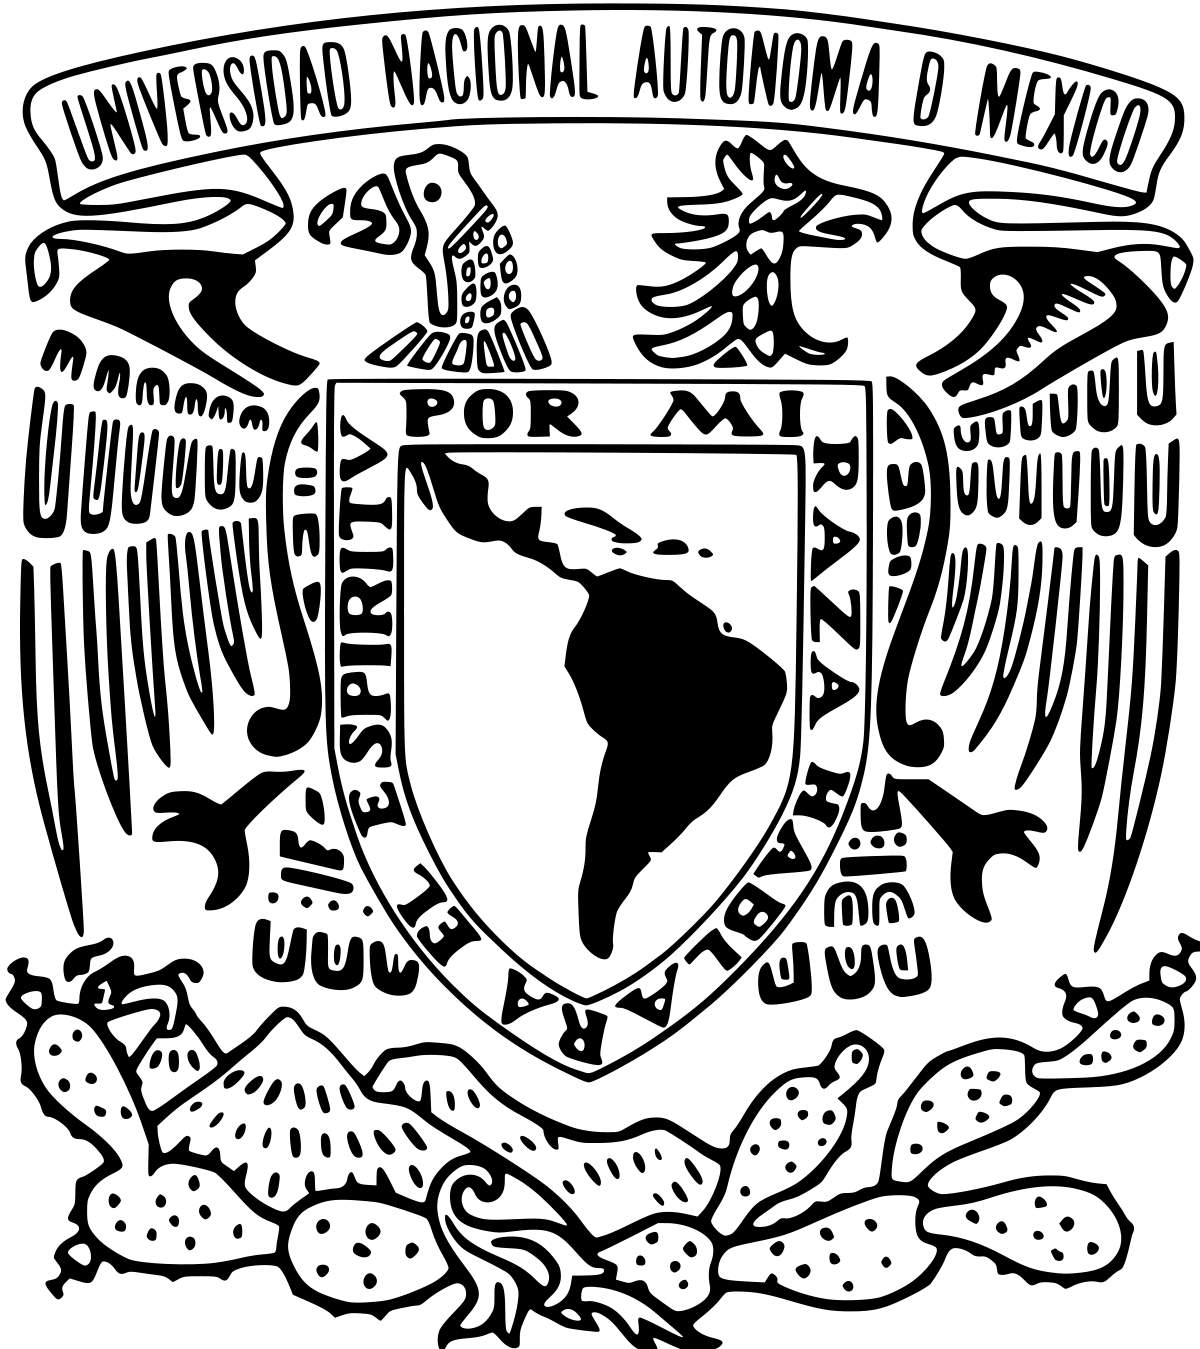
\includegraphics[height = 0.14\textheight]{recursos/Logo_UNAM.png}\par
    	\end{center}
    \end{minipage}\hfill
    \begin{minipage}{10cm}
    	
    \end{minipage}\hfill
    \begin{minipage}{3cm}
    	\begin{center}
    		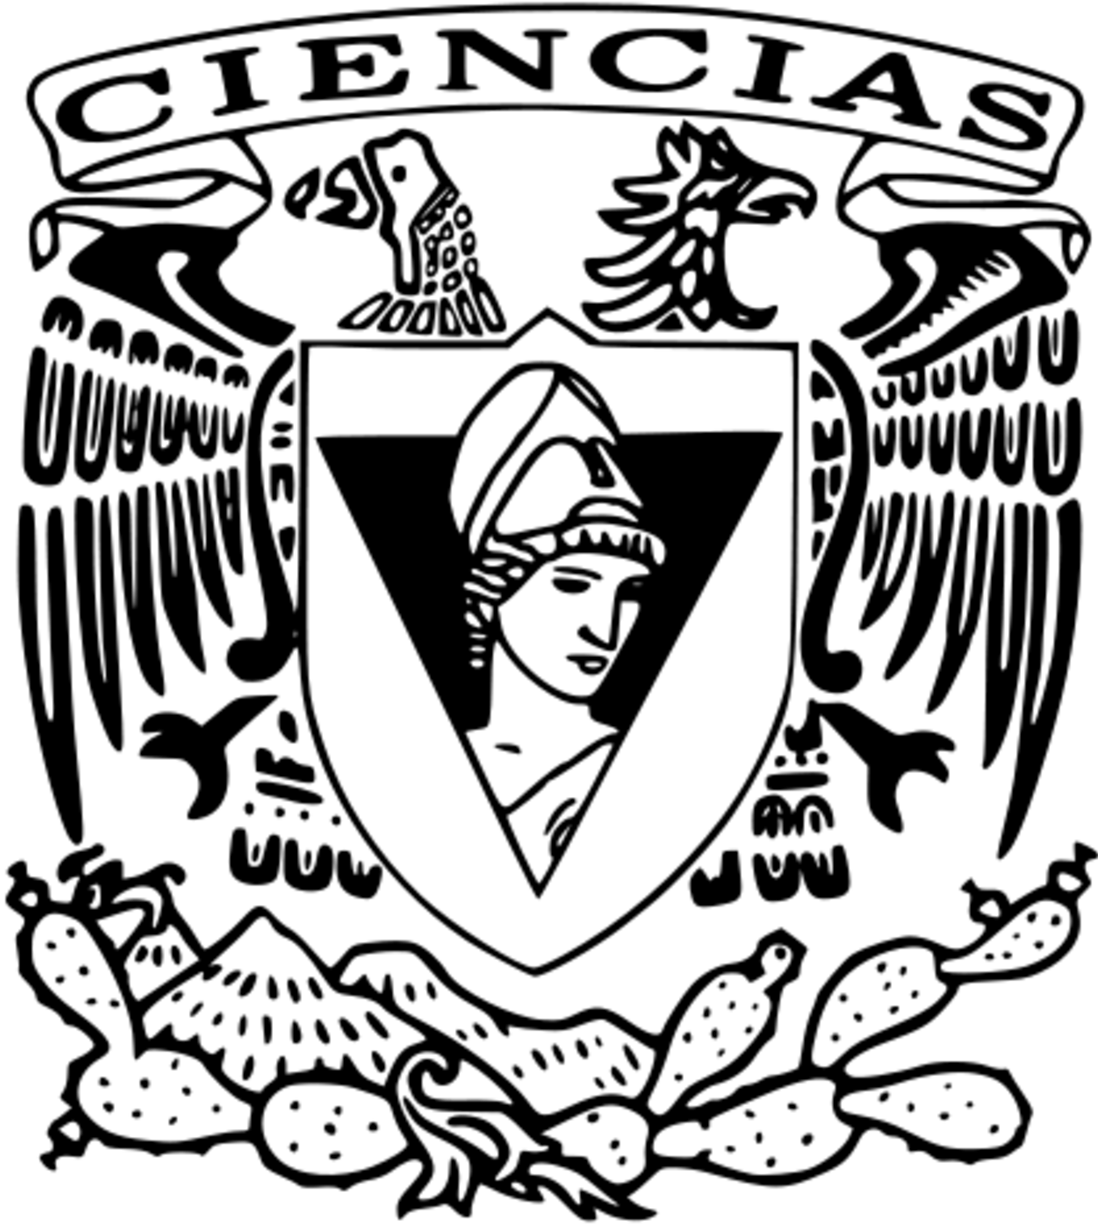
\includegraphics[height = 0.14\textheight]{recursos/Logo_FC.png}\par
    	\end{center}
    \end{minipage}
        \centering
        \vspace{1cm}
        
        {\bfseries\LARGE Universidad Nacional Autónoma de México \par}
        
        \vspace{1cm}
        {\scshape\Large Facultad de Ciencias \par}
        \vspace{1cm}
        {\scshape\Large Estructuras Discretas \par}
        \vspace{1cm}
        {\scshape\Large Licenciatura en Ciencias de la Computación \par}
        \vspace{1cm}
        {\scshape\Huge Tarea 01: Naturales, inducción y recursión  \par}
        \vspace{3cm}
        {\itshape\Large Primer Parcial \par}
        \vfill
        {\Large Autores: \par}
        {\Large Ramírez Mendoza Joaquín Rodrigo \par}
        {\Large Villalobos Juárez Gontran Eliut\par}
        {\Large Treviño Puebla Héctor Jerome \par}
        \vfill
        {\Large Agosto 2024 \par}
    \end{titlepage}
% ---Fin de la portada de la portada
    \maketitle

% Introducir aquí sus capítulos
% ------

\end{document}